\chapter{Final Discussion and Future Steps} \label{ch:Final Discussion and Future Steps}
Our investigation reveals that while human and bovine \textit{IFITs} exhibit differential induction upon RSV infection, both human and bovine IFIT proteins are detectable in cells during RSV infection, indicating their potential to exert anti-RSV activity. Upon conducting a comprehensive analysis of IFIT protein interactions with RSV inclusion bodies and pseudo-inclusion bodies, we observed interaction phenotypes across all IFITs, implying their association with these structures. However, it is noteworthy that we have not assessed the propensity of any cytosolic protein to interact with these structures, posing a significant limitation to this study. This could be addressed by expressing inert, easily visualised proteins like GFP or staining for a panel of endogenous cellular proteins with different sizes, molecular polarities, and structural motifs. Such an approach would provide insights into how a diverse range of unrelated proteins interact with these structures. Furthermore, our analysis faces limitations due to the maximal resolution of images obtained through confocal microscopy. Colocalisation and edge exclusion phenotypes may be technical artefacts, possibly arising from IFITs being adjacent to the IB structures or mislabelled diffusion phenotypes. To alleviate these concerns, the use of super-resolution microscopy methodologies, which surpass natural diffraction limits and lead to resolving entities which are less than 250 nm apart, could be employed \cite{Schermelleh2019Super-resolutionDemystified}. The final analysis in this project, assessing the interaction phenotypes of exogenously expressed IFIT proteins concerning RSV inclusion bodies in co-infected/transfected cells, heavily relied on cell permissivity for infection and subsequent transfection. This introduced an inherent bias, as the majority of infected cells were non-permissive to subsequent transfection, making the observed co-infected/transfected cells more likely outliers than representative of normal cell behaviour. Additionally, the methodology resulted in low co-infection/transfection efficiencies, limiting the number of observations. These issues could be addressed by establishing IFIT-expressing cell lines based on permissive cells for RSV infection and suitable for confocal microscopy, such as the A549 cell line. Potential disruptions to cellular homeostasis by IFIT proteins, including promotion of apoptosis (IFIT2), cell cycle arrest (IFIT3), and general reduction of cellular translation (IFIT1), could be mitigated by creating inducible cell lines. The inducible expression could be activated just before, during, or after RSV infection \cite{Kallunki2019HowStudies}. This approach not only provides more opportunities to observe exogenous IFIT and RSV interactions but also allows assessment of whether the IFIT anti-RSV function is temporally restricted to a specific phase of RSV infection.

Drawing upon the accumulated information, we propose a model elucidating the response of IFITs to RSV infection. RSV entry and successful replication trigger heightened interferon production and secretion from infected cells, thereby elevating interferon-stimulated gene expression in neighbouring cells. Among these genes, \textit{IFITs} are expressed, creating a preventative anti-RSV antiviral environment. This inference is supported by the findings in Chapter \ref{ch:Assessment of Transcriptional Induction of Human IFITs in the Context of RSV}, wherein the induction of human \textit{IFITs} by hRSV is impeded by an interferon receptor inhibitor and halted when hRSV is UV-crosslinked, rendering it incapable of replication. Upon infiltration of initially uninfected cells by RSV, either through syncytia formation or entry of RSV particles, IFIT proteins interact with RSV inclusion bodies with distinct dynamics. These are summarised by Figure \ref{fig:Final Thesis Figure.}. We propose a model where IFIT1 and IFIT5 exhibit a propensity to translocate to and interact with RSV inclusion bodies. However, certain mechanisms mediated by RSV proteins, excluding N and P, actively prevent their access. This is inferred from our previous observations, where endogenous IFIT1 and IFIT5 initially exhibited low proportions of strong interaction phenotypes with RSV IBs during infection, significantly increasing in the context of RSV pIBs. Moreover, increased concentrations of IFIT1 and IFIT5 during RSV infection correlated with an increased occurrence of strong interaction phenotypes. Furthermore, we posit the existence of a subpopulation of IFIT2, potentially differentiated by its presence in a C-terminal-enabled heteromeric configuration with other binding partners. Interaction with these partners, abundant under homeostatic conditions, but reducing in abundance during RSV infection, consistently leads to IFIT2 associating with RSV inclusion bodies. However, this association is contingent upon the abundance of the interaction partner. Thus, if the concentration of IFIT2 increases without a corresponding increase in the quantity of the binding partner, the overall frequency of IFIT2 association with RSV IBs diminishes. This hypothesis is grounded in our previous findings, where the IFIT2(A) antibody consistently demonstrated a strong association of IFIT2 with both RSV IBs and pIBs, while the IFIT2(B) antibody consistently exhibited an exclusion interaction phenotype. Since the IFIT2(A) antibody was raised against an antigen encompassing almost the entire length of IFIT2, and the IFIT2(B) antibody was raised against only the N-terminal of IFIT2, we infer that the differential staining pattern is linked to the C-terminus of IFIT2. Additionally, staining for exogenous IFIT2-FLAG using the anti-FLAG antibody in the context of RSV pIBs unveiled the proportion of strong interaction phenotypes and exclusion, as individually identified by IFIT2(A) and IFIT2(B) antibodies. Conversely, detection of exogenous IFIT2-FLAG using the anti-FLAG antibody in the context of RSV infection reveals a decreased association of IFIT2 with RSV IBs. Moreover, we propose that a proportion of IFIT3 associates with RSV IBs, dependent on cellular binding partners whose abundance remains stable between control and infected cells. The foundation of this hypothesis lies in the stable frequencies of strong interaction phenotypes observed between RSV IBs and pIBs and endogenous and exogenous IFIT3.

\begin{figure}
    \centering
    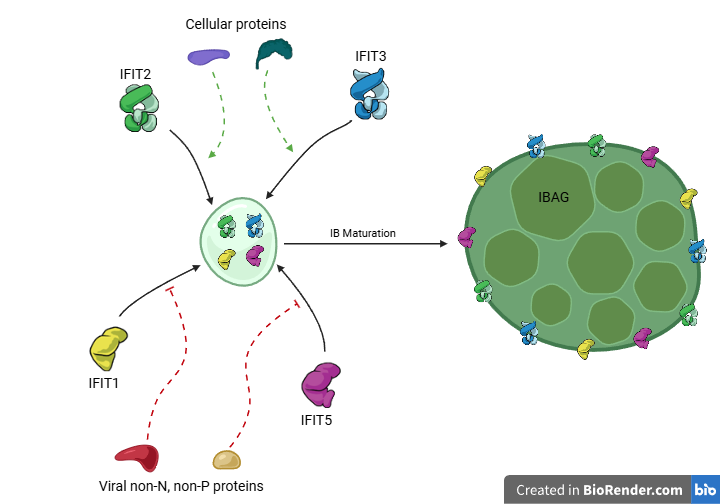
\includegraphics[width=0.7\linewidth]{10. Discussion and Conclusion/Final Thesis Figure.png}
    \caption[Proposed Model of IFIT Interaction with RSV Inclusion Bodies.]{\textbf{Proposed Model of IFIT Interaction with RSV Inclusion Bodies.} Depicted is a proposed model of IFIT interaction with RSV inclusion bodies. IFIT1 and IFIT5 exhibit a propensity to translocate to and interact with RSV inclusion bodies. However, certain mechanisms mediated by RSV proteins, excluding N and P, actively prevent their access. Furthermore IFIT2 and IFIT3 are able to interact with RSV inclusion bodies only when certain non-specified cellular binding partners are present. Lastly, all IFITs undergo a staged progression of inclusion body association. Initially, they are located within small, immature IBs, and as these structures mature, they increase in size and give rise to the inclusion body-associated granules. Subsequently, IFITs translocate to the inclusion body boundary. Created with BioRender.com.}
    \label{fig:Final Thesis Figure.}
\end{figure}

Finally, we postulate that IFITs collectively undergo a staged progression of inclusion body association. Initially, they are located within small, immature IBs, and as these structures mature, they increase in size and give rise to the inclusion body-associated granules. Subsequently, IFITs translocate to the inclusion body boundary where the RSV genome is situated. This comprehensive process culminates in the reduction of the maximal size and alteration of the normal physiology of RSV IBs. It is plausible that during the formation of inclusions within immature IBs, IFIT proteins negatively influence viral RNA synthesis, leading to the inhibition of IB maturation. Exploring this potential effect of IFIT proteins could be achieved through the use of the RSV minigenome system. In the RSV minigenome system, a synthetic RSV genome, consisting of reported genes located between the 3$^{\prime}$ and 5$^{\prime}$ ends of the viral RNA, is transfected into mammalian cells along with components of the RSV polymerase complex, namely N, P, M2/1, and L proteins \cite{Teng2016UseTranscription}. This methodology provides a controlled assessment of the impact of restriction factors, such as IFIT proteins, on RSV viral translation and replication. Employing the minigenome system in the context of exogenously expressed IFITs would enable a quantitative evaluation of the extent to which these proteins influence viral RNA synthesis. Moreover, it is imperative to investigate the specific interactions between IFIT proteins and RSV proteins. Oliveira \textit{et al.} previously examined the interactions of exogenously expressed hRSV N, P, and M proteins with the HEK293T cellular proteome using immunoprecipitation coupled with mass spectrometry methodologies. Intriguingly, neither of the IFIT proteins emerged as potential interactors in that study \cite{Oliveira2013HumanCells}. This suggests that other RSV proteins may be accountable for the hypothesised influence of IFIT interaction with RSV inclusion bodies, or alternatively, our hypothesis may need reassessment. Addressing this could be achieved through the same methodology, i.e., immunoprecipitation coupled with mass spectrometry, where we would identify IFIT interaction partners during RSV infection.

In summary, this doctoral thesis unveils differential induction of human and bovine \textit{IFITs} during RSV infection, affirming their detectability in cells and potential anti-RSV activity. A proposed model outlines the orchestrated response of IFITs to RSV, initiated by heightened interferon production post-RSV entry. Notably, IFIT1 and IFIT5 exhibit a proclivity for RSV inclusion bodies, influenced by RSV proteins, while IFIT2 demonstrates dynamic interactions dependent on C-terminal configurations and partner abundance. The staged progression of IFIT inclusion body association suggests a nuanced role in altering RSV inclusion body physiology, however, employing the RSV minigenome system for controlled assessments and exploring specific IFIT-RSV protein interactions via immunoprecipitation and mass spectrometry are imperative for advancing our understanding. Thus our study illuminates species-specific responses of human and bovine \textit{IFITs} to RSV infection, offering insights for targeted antiviral strategies. The proposed model unveils orchestrated host immune responses, emphasising \textit{IFITs} in establishing a preventative antiviral environment. Understanding IFIT interactions with RSV inclusion bodies informs potential targets for antiviral drug development. Overall, our findings deepen comprehension of host-virus dynamics, paving the way for precise interventions to combat RSV and other viral infections.

%Words in text: 1374
%Words in headers: 5
%total = 1379
% total words: 100 + 509 + 484 + 6,457 + 4,015 + 5,732 + 4,338 + 8,965 + 13,797 + 1,379 = 45,476
% total figures: 8 + 5 + 13 + 13 + 34 + 60 = 133